% Please do not change the document class
\documentclass{scrartcl}

% Please do not change these packages
\usepackage[hidelinks]{hyperref}
\usepackage[none]{hyphenat}
\usepackage{setspace}
\usepackage{graphicx}
\doublespace

% You may add additional packages here
\usepackage{amsmath}
\usepackage{multicol}
\usepackage{multirow}
\usepackage{array}

% Please include a clear, concise, and descriptive title
\title{Usability Analysis}

% Please do not change the subtitle
\subtitle{COMP140 - Usability Analysis}

% Please put your student number in the author field
\author{1507290}

\begin{document}

\maketitle

\abstract{}



\section{Introduction}

This report will analyse the usability issues raised in an evaluation of a controller designed for \textit{Hotrod the Beetle} concerning its use of LEDs and its interaction with the game.

\section{The Controller}
The controller is used by rotating a disc with an image of Hotrod on so that he is facing in the direction of intended travel. An image of the controller is shown in Figure~\ref{fig:controller}.
\begin{figure}
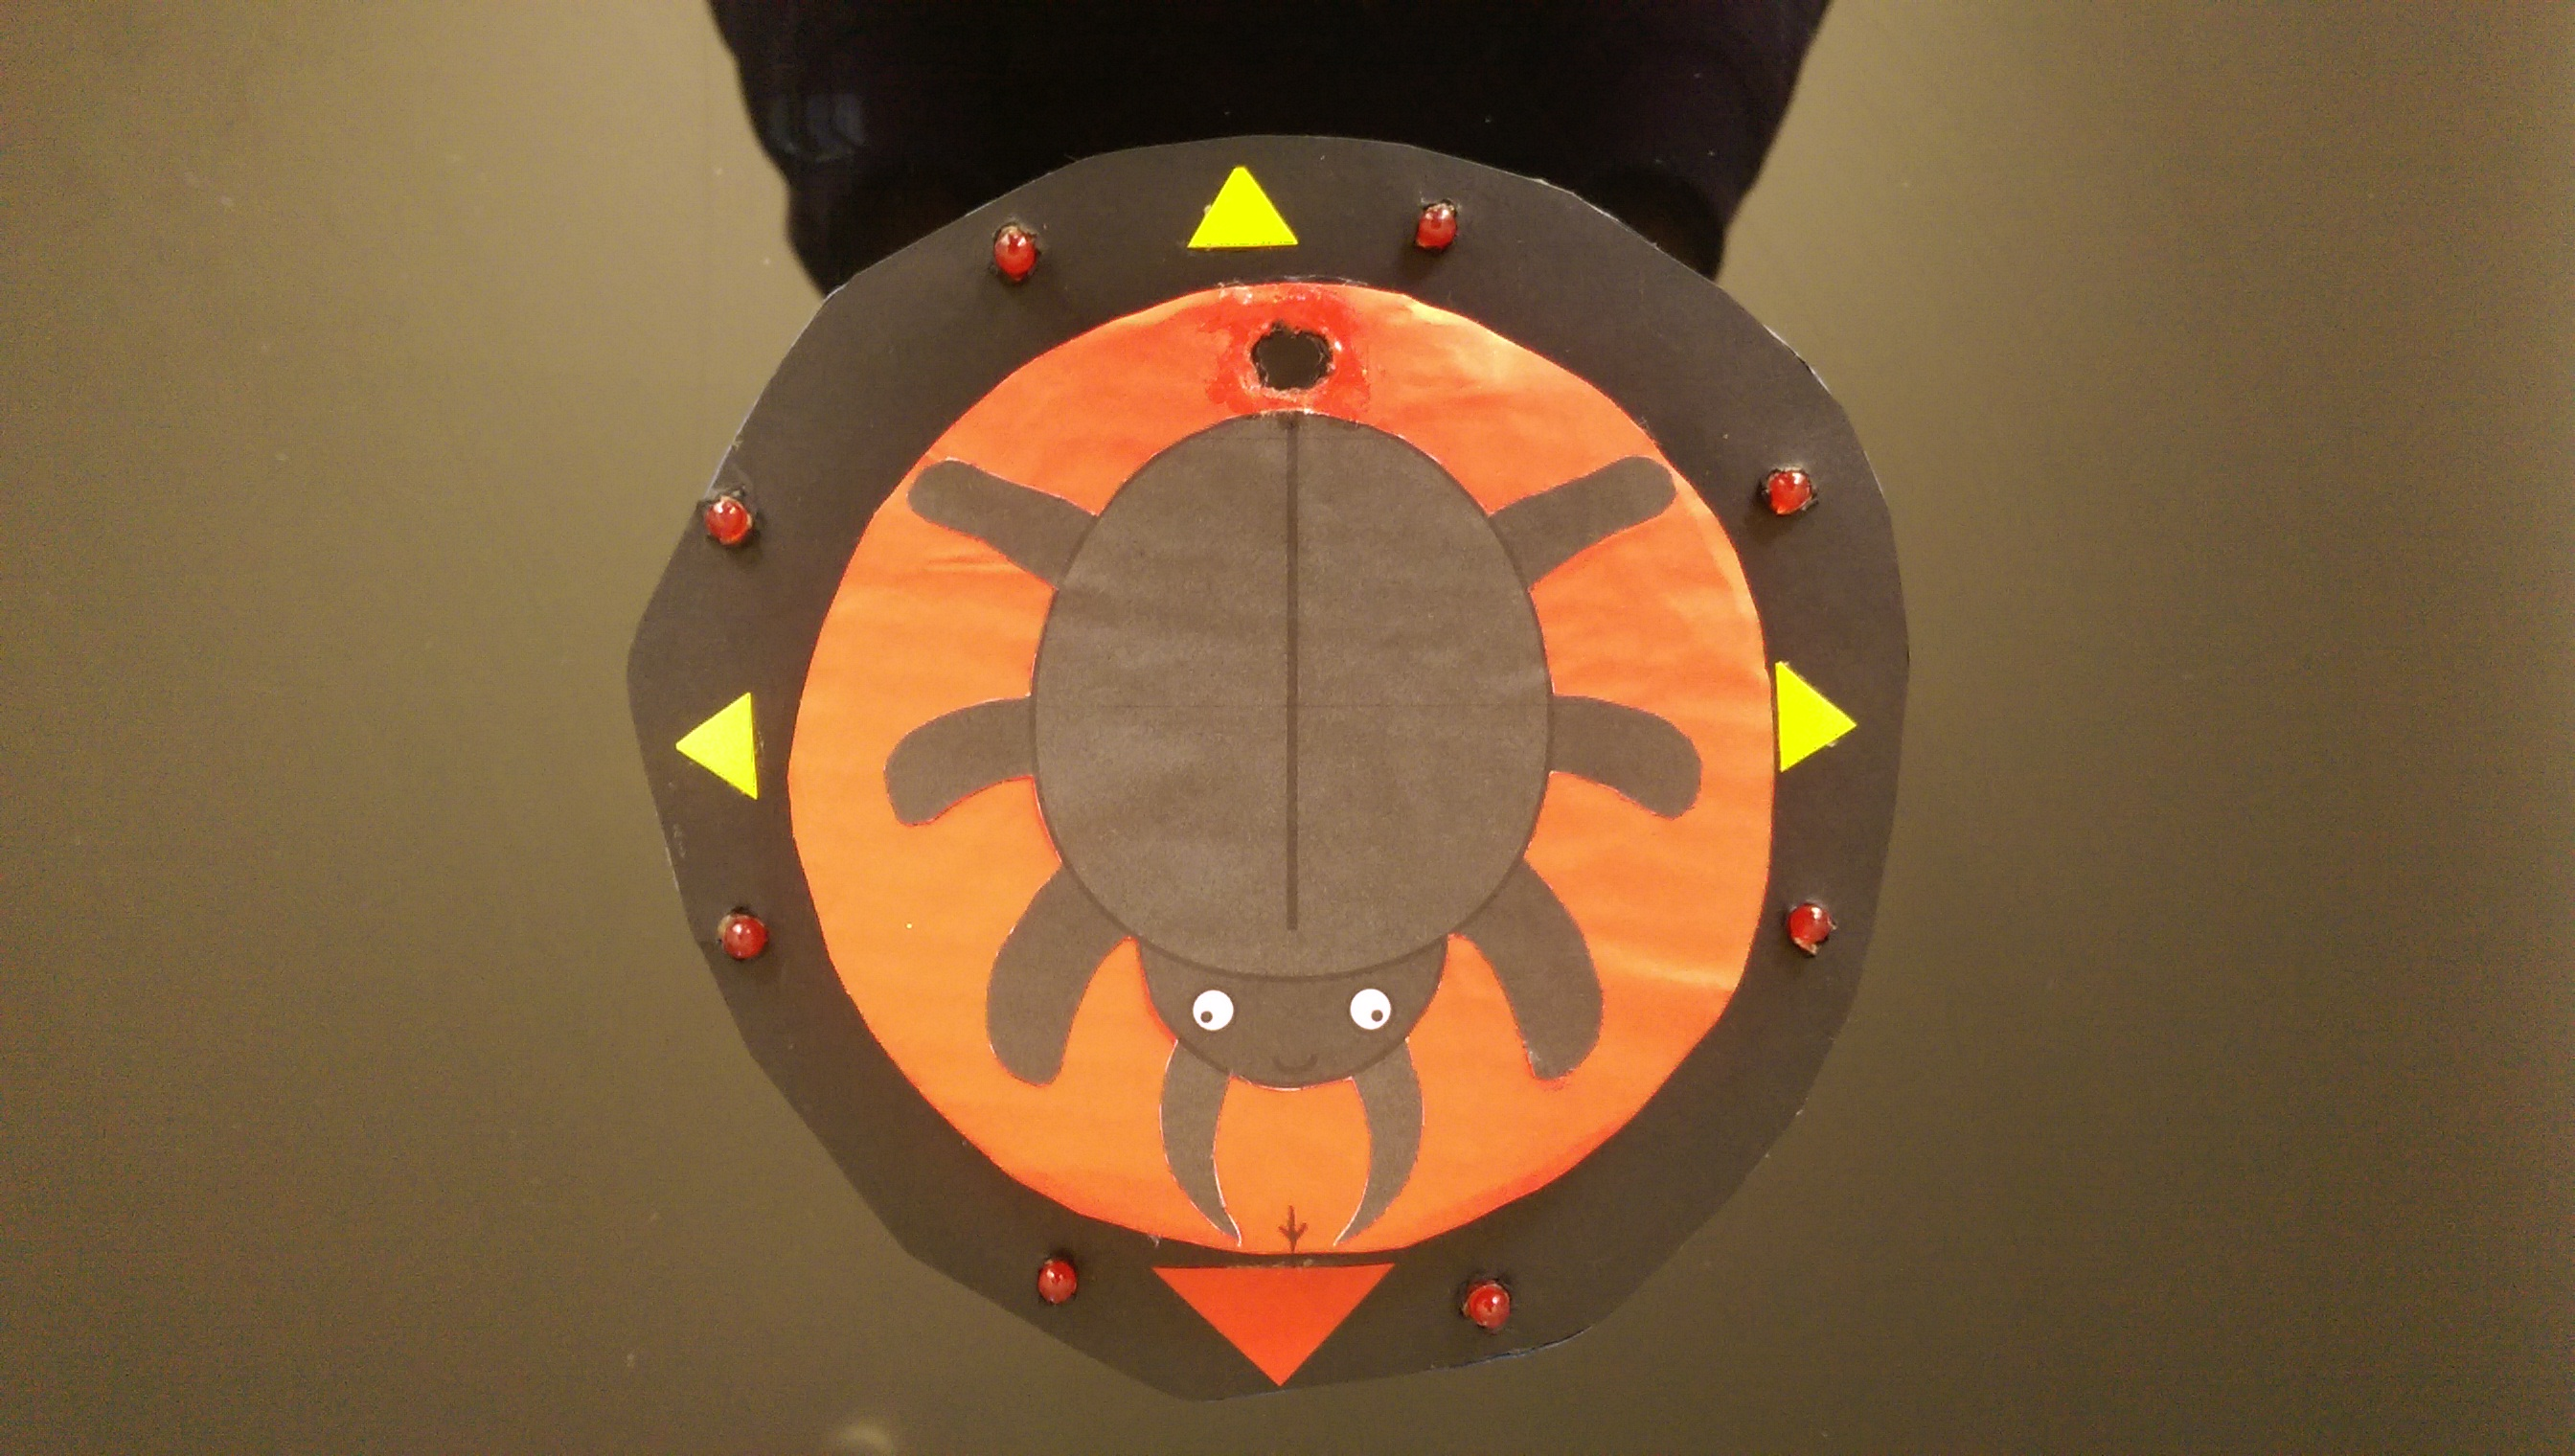
\includegraphics[width=\textwidth]{controller.jpg}
\caption{The Hotrod game controller}
\label{fig:controller}
\end{figure} 

\begin{table}
\centering
\begin{tabular}{| l | p{6cm} |}
\hline
\textbf{Heuristic} & \textbf{Application to Game Controller} \\ \hline
Responsiveness of controls & Inputs on the controller should be reflected promptly in the game \\ \hline
Ease of interpretation of system status & The status of the game and the controller should be made clear and easy to interpret without distracting from the game \\ \hline
Recognition over recall & The functions of each component of controller should be easily recognisable, rather than needing to remember what each button does or what each light represents. The player should be able to process information with minimal cognitive effort.\\ \hline
Clear and simple design & The controller should require minimal instruction. The way it is used should be intuitive, and it should not convey any unneeded information.\\ \hline
\end{tabular}
\caption{Heuristics used in the usability analysis of the controller}
\label{table:heuristics}
\end{table}


\section{Evaluation Process}
Due to the circumstances of the review session, the controller was only reviewed by one evaluator. As a result, it is likely that there will be further usability problems that were not reported by the evaluator. The review would have been more effective if there were between three and five evaluators~\cite{nielsen:evaluation}. The review process was otherwise carried out by following the guidelines provided by Nielsen~\cite{nielsen:how}.

\section{Heuristics}
The heuristics used are described in Table~\ref{table:heuristics}. They are adapted from Nielsen's heuristics~\cite{nielsen:heuristics} and Pinelle's heuristics~\cite{pinelle:heuristic} in order to be made more appropriate for the analysis of a game controller.

\section{Design Issue 1: Purpose of LEDs Unclear}
The reviewers indicated that the purpose of the LEDs was unclear, as described in Table~\ref{table:issue1}. The LEDs indicate where the walls are. Their use was likely unclear as they do not enhance the gameplay or provide the player with any useful information. The player often won't have time to look down at the controller. Furthermore, the information that the LEDs are intended to convey is displayed on-screen in a clearer and more helpful manner.

\subsection{Proposed Solutions}
The reviewer reported initially believing that the LEDs were indicating the orientation of the controller. This may indicate that this is a more intuitive and clear use of the LEDs. Furthermore, providing an indication of the direction the controller is registering will be more useful to the player, as it can sometimes be unclear which direction is active due to the nature of the controller's free rotation. 

An even more effective use of the LEDs could be to flash when the player is powered up. This could be registered in the player's peripheral vision without requiring them to look away from the screen and process complex information.

\begin{table}[h]
\centering
\begin{tabular}{|m{5cm}|m{6cm}|}
\hline
\textbf{Heuristic} & \textbf{Observation} \\ \hline
Recognition over recall \par Clear and simple design & 
By the time the information that the LEDs are conveying has been processed, the state of the game has changed. This information is both unnecessary and distracting, as it is available on-screen in a more helpful form. The LEDs should convey simpler information that doesn't require the player to look away from the game. \\ \hline
Ease of interpretation of system status & 
The LEDs are difficult to interpret. Their purpose is not obvious without explicitly being told. They distract from the game as the player must look away in order to make sense of them. This makes it harder to relate the information they provide to the game, as the game's state is constantly changing. \\ \hline
\end{tabular}
\caption{Observations relating to heuristics relevant to \textit{Design Issue 1: Purpose of LEDs Unclear}}
\label{table:issue1}
\end{table}

\section{Design Issue 2: Controls Feel Unresponsive}
The controller was reported to feel unresponsive: you must rotate the controller \textit{before} the desired turning, otherwise the character will continue past. The observations are described in Table~\ref{table:issue2}. This could be caused by a disconnect between the game's design and the controller's design. The game compensates for the character's continuous movement by allowing input to be registered before a turning. Not only is this the optimal way to play, but the time taken to physically manipulate the controller means that this play-style is enforced. However, this results in an inconsistency between the controller's image and the game's image.

\subsection{Proposed Solutions}
It may not be appropriate to change the way the game responds to input, as this would reduce the responsiveness and control provided when playing the game using different control methods. Therefore, reducing the controller's size so that the distance it needs to travel to rotate is smaller may help increase the feeling of responsiveness. The image of Hotrod still won't correspond to the image on screen most of the time, but it can be perceived as instructing him where to go next.

\begin{table}[h]
\centering
\begin{tabular}{| l | p{6cm} |}
\hline
\textbf{Heuristic} & \textbf{Observation} \\ \hline
Responsiveness of controls
 & The controller creates a feeling of unresponsiveness. It feels natural to turn the controller at the time the character is intended to turn. However, doing this results in the movement not being registered until after the turning. \\ \hline
Ease of interpretation of system status
 & The way the controller should be used is confusing. If the optimal play-style is used, the controller does not match what is seen on screen. This makes the player feel that turning the controller at the instant a direction change is desired is how it should be used, resulting in issues concerning lack of responsiveness. \\ \hline
\end{tabular}
\caption{Observations relating to heuristics relevant to \textit{Design Issue 2: Controls Feel Unresponsive}}
\label{table:issue2}
\end{table}

\section{Conclusion}
The usability of the controller may be increased by applying the proposed changes to the design in order to address the issues raised during the evaluation.

\bibliographystyle{ieeetran}
\bibliography{comp140-evaluation}

\end{document}
